\subsection{Élaboration du diagramme de Gantt} 
Un diagramme de Gantt a été élaboré pour planifier et suivre les différentes étapes du projet. Voici un aperçu des principales étapes du projet :
\begin{itemize}
    \item \textbf{Analyse des besoins} : Compréhension des objectifs du projet et des données disponibles.
    \item \textbf{Collecte des données} : Récupération des données nécessaires à l'analyse.
    \item \textbf{Nettoyage et préparation des données} : Traitement des données pour les rendre exploitables.
    \item \textbf{Analyse exploratoire des données (EDA)} : Exploration des données pour identifier les tendances et les anomalies.
    \item \textbf{Modélisation et analyse prédictive} : Développement de modèles pour prédire les résultats futurs.
    \item \textbf{Visualisation des données} : Création de graphiques et de tableaux de bord pour présenter les résultats.
    \item \textbf{Rédaction du rapport final} : Compilation des résultats et rédaction du rapport de stage. 
    voici un aperçu du diagramme de Gantt :
    \begin{center}
    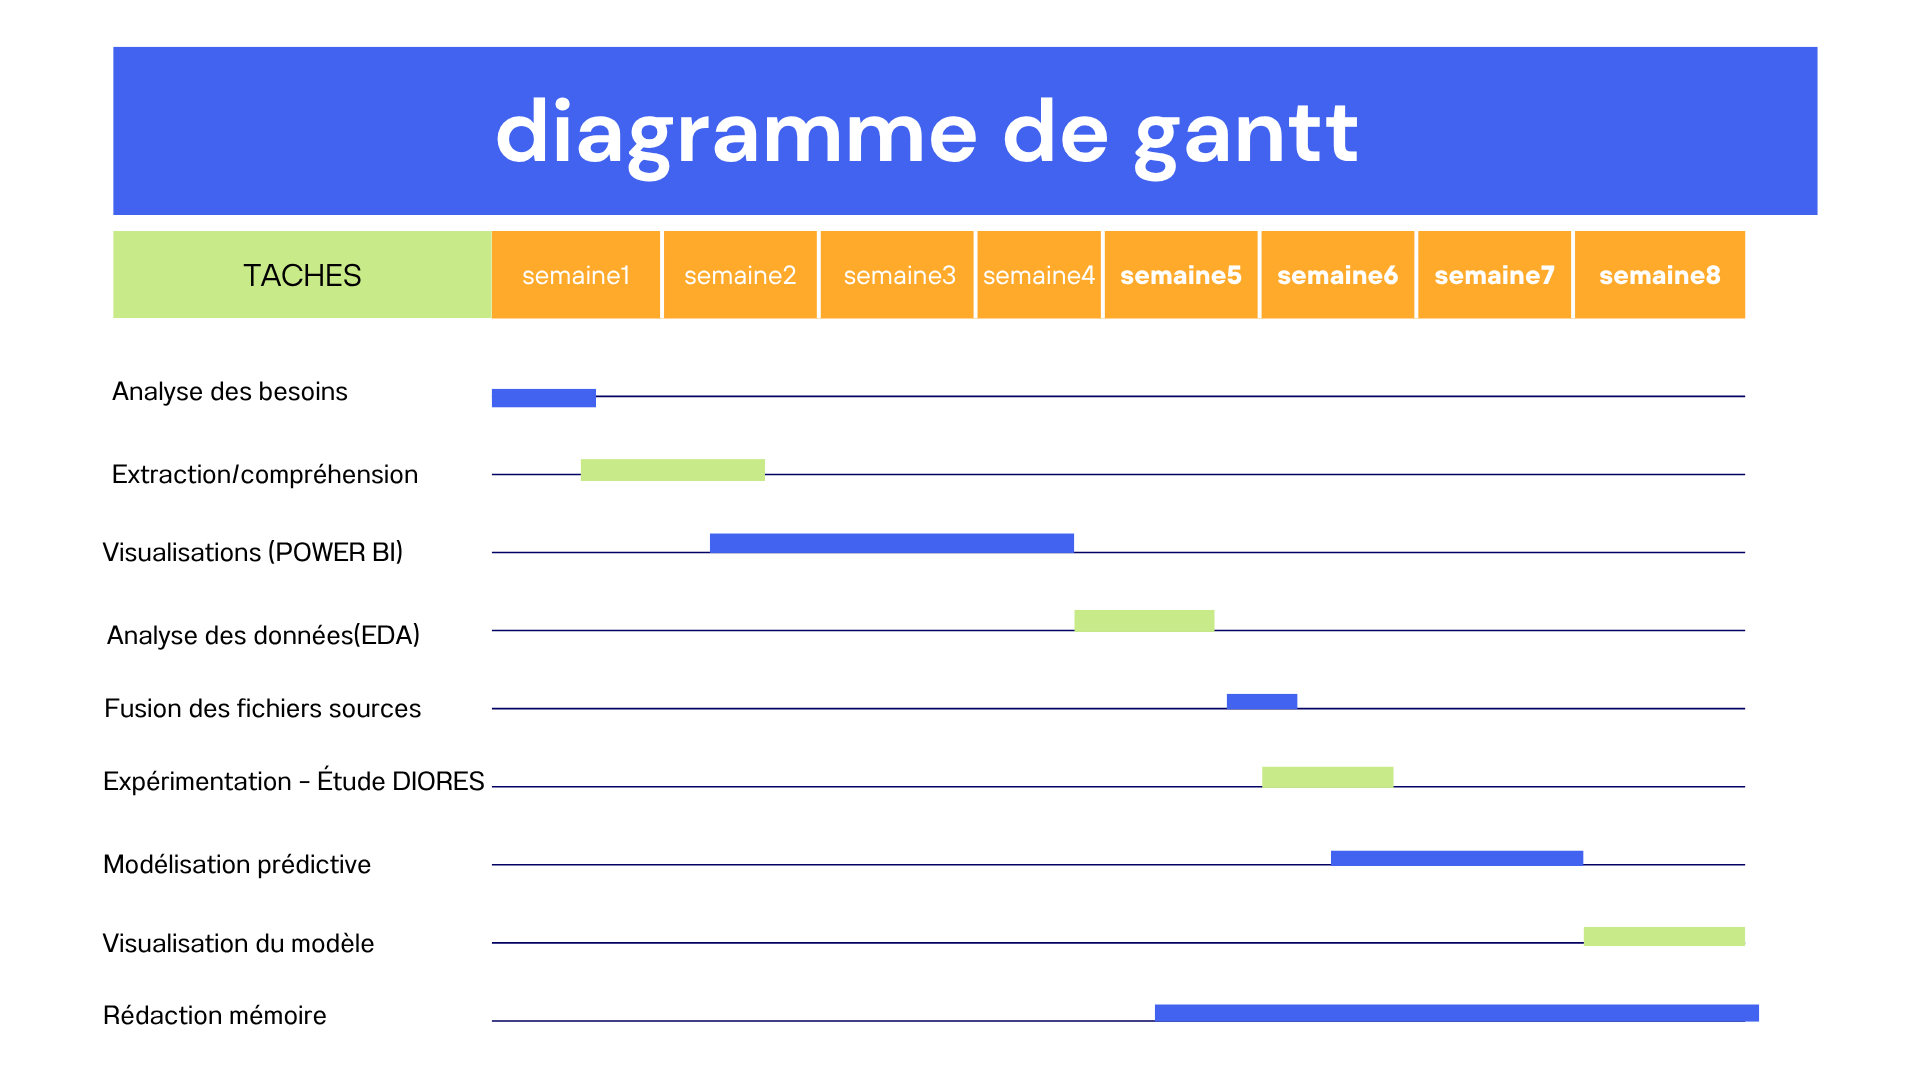
\includegraphics[width=1\textwidth]{image/Gantt.png} 
    \end{center}

\end{itemize} 

\subsection{Extraction et compréhension des données} 
Les données utilisées pour mon stage ont été extraites d'un entrepôt de données de l'Université appelé RADIS. Une fois extraites, les données ont été ouvertes sur plusieurs outils comme Excel et Power BI pour une première compréhension. Ensuite, elles ont été importées dans Python pour avoir un premier aperçu des données et faire les premiers filtres. 

Pour bien comprendre les données, mon encadrant m'a demandé de faire plusieurs tâches comme : 
\begin{itemize}
    \item \textbf{Se rendre à la DISI} : Mon encadrant m'a demandé de me rendre à la DISI (Direction de l'informatique et des systèmes d'information) pour comprendre comment les données sont stockées, ce que signifie chaque colonne, et enfin prendre conscience des données disponibles pour des analyses futures.  
    \item \textbf{Détection d'anomalies} : Une fois toutes les colonnes des données comprises, j'ai créé un fichier pour détecter les anomalies et incohérences dans les données. J'ai utilisé des outils comme Excel pour des filtres et des tableaux croisés dynamiques, ainsi que Python pour des analyses plus approfondies. 

    Cette fonction prend en entrée un fichier de données CSV et retourne un fichier texte avec toutes les incohérences.  
    Ce fichier, qui contient ces anomalies et incohérences, a été transmis à mon encadrant et à la DISI pour qu'ils puissent corriger les données.

    Cette tâche m'a permis de mieux comprendre les données et de m'assurer de leur qualité avant de procéder à l'analyse. J'ai aussi appris comment les données sont stockées et comment elles peuvent être utilisées pour des analyses futures.  
    La difficulté de cette tâche était de comprendre les données et de détecter les anomalies, car les données étaient volumineuses et complexes. Cependant, j'ai réussi à surmonter cette difficulté en utilisant des outils comme Excel et Python pour filtrer et analyser les données.

    \item \textbf{Transformation des données} : Conversion des types de données, normalisation et agrégation des données pour les rendre exploitables. 
\end{itemize}

\subsection{Visualisation des données avec Power BI}  
Power BI a été utilisé pour créer des visualisations interactives des données. J'ai travaillé avec mon collègue qui avait déjà commencé à faire des visualisations sur Power BI. J'ai donc continue a travailler avec lui et on a réussi a faire plusieurs tableau de bord 
On a  créer plusieurs graphiques et tableaux de bord pour présenter les résultats de l'analyse des données. Voici quelques exemples de visualisations que on a  créées : 
\begin{itemize}
    \item \textbf{Tableaux de bord des étudiants } : On a créer un Tableau de bord  des étudiants avec plusieurs graphiques et filtres pour explorer les données des étudiants par exemple pour chaque année le nombre d'étudiants inscrit homme et femme, le nombre d'étudiants pour chaque système LMD ou classique et pour chaque niveau (L1, L2 , 1A, 2A .....) , l'evolution des effectifs des étudiants au fil des années , le nombre d'étudiants inscrits pour chaque faculté , ecole , Institut et ecole doctorale. Voici quelques insights que nous avons pu obtenir à partir de ces visualisations : 
    
    - le nombre d'étudiants inscrits a augmenté au fil des années, avec une tendance à la hausse significative. on compte plus de 80000 étudiants inscrits pour l'année académique 2023-2024. 

    - 50\% des étudiants sont inscrits a la faculté des lettres et sciences humaines (FLSH) et la faculté des sciences et techniques (FST) 

    - La majorité des étudiants sont inscrits en L1, suivis de L2 et L3. 
    
    - l'ecole avec le plus d'étudiants  est L'ESP avec plus de 5000  inscrits pour l'année académique 2023-2024.

    - la reparation d'hommes et femmes est presque égale, avec 
    une légère majorité d'hommes 47000 hommes contre 41000 femmes pour l'année académique 2023-2024. 

    Voici un aperçu du tableau de bord des étudiants :
    
    \begin{center}
    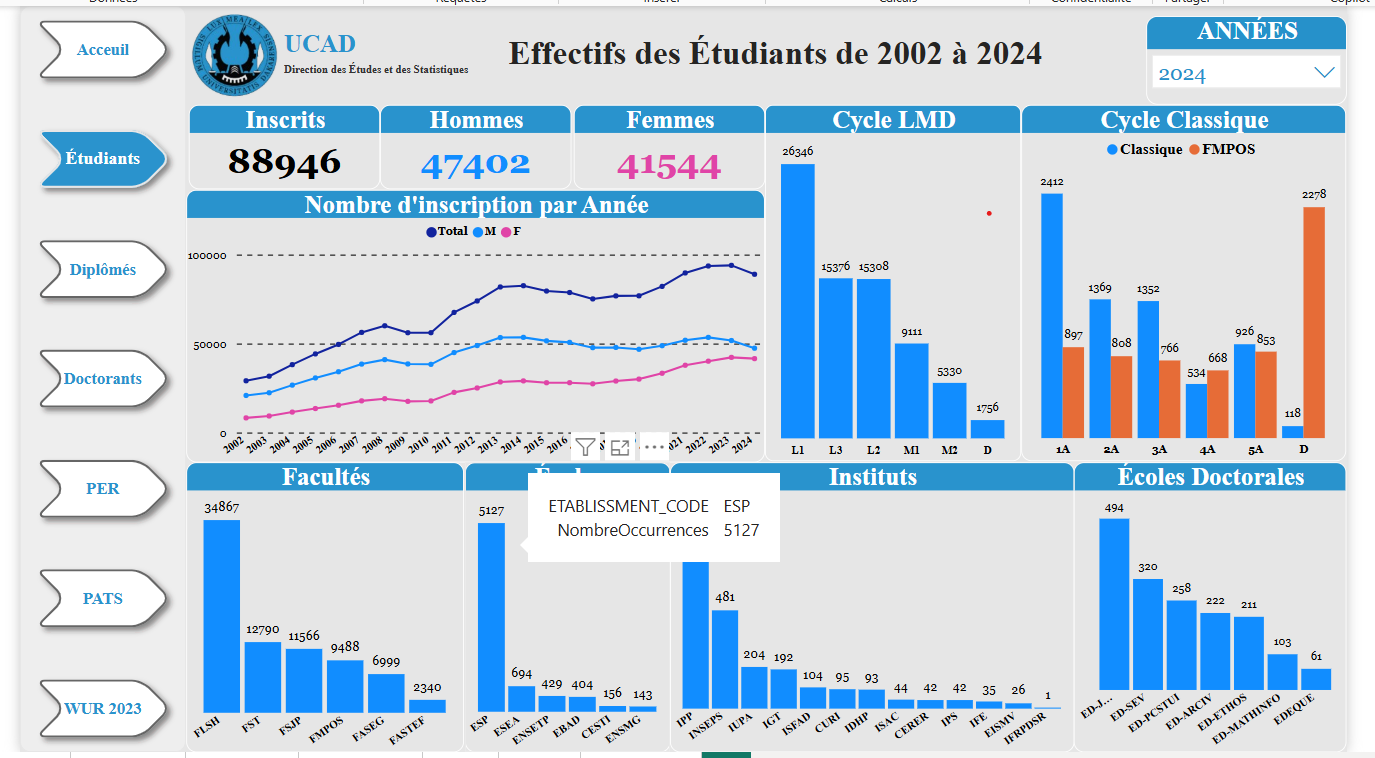
\includegraphics[width=1\textwidth]{image/etudiants.png} 
    \end{center}


    \item \textbf{Tableaux de bord des diplômes} : Dans cette sections plusieurs graphiques ont été créés pour explorer les données des diplômes obtenus par les étudiants. On a pu créer des graphiques pour visualiser le nombre de diplômes obtenus par année, par faculté, par niveau d'étude . Voici quelques insights que nous avons pu obtenir à partir de ces visualisations :
    
    - le nombre de diplômés a diminuer entre  2016 et 2017 et est devenu constante  jusqu'a 2021, avec une moyenne de 5000 diplômes (license et Master) par an et une légère augmentation en 2022 et 2023.

    - La majorité des diplômes sont issus de la la FLSH ce qui normalement est dû au nombre élevé d'étudiants inscrits dans cette faculté Cependant on remarque parmi ces diplômes, la majorité sont des licences et que ils sont constitue de 60\% de femmes et 40\% d'hommes.

    - Par contre avec l'ensemble des diplômes obtenus, on remarque que la majorité sont des hommes, avec 53\% d'hommes et 47\% de femmes. 

    Voici un aperçu du tableau de bord des diplômes :

    \begin{center}
    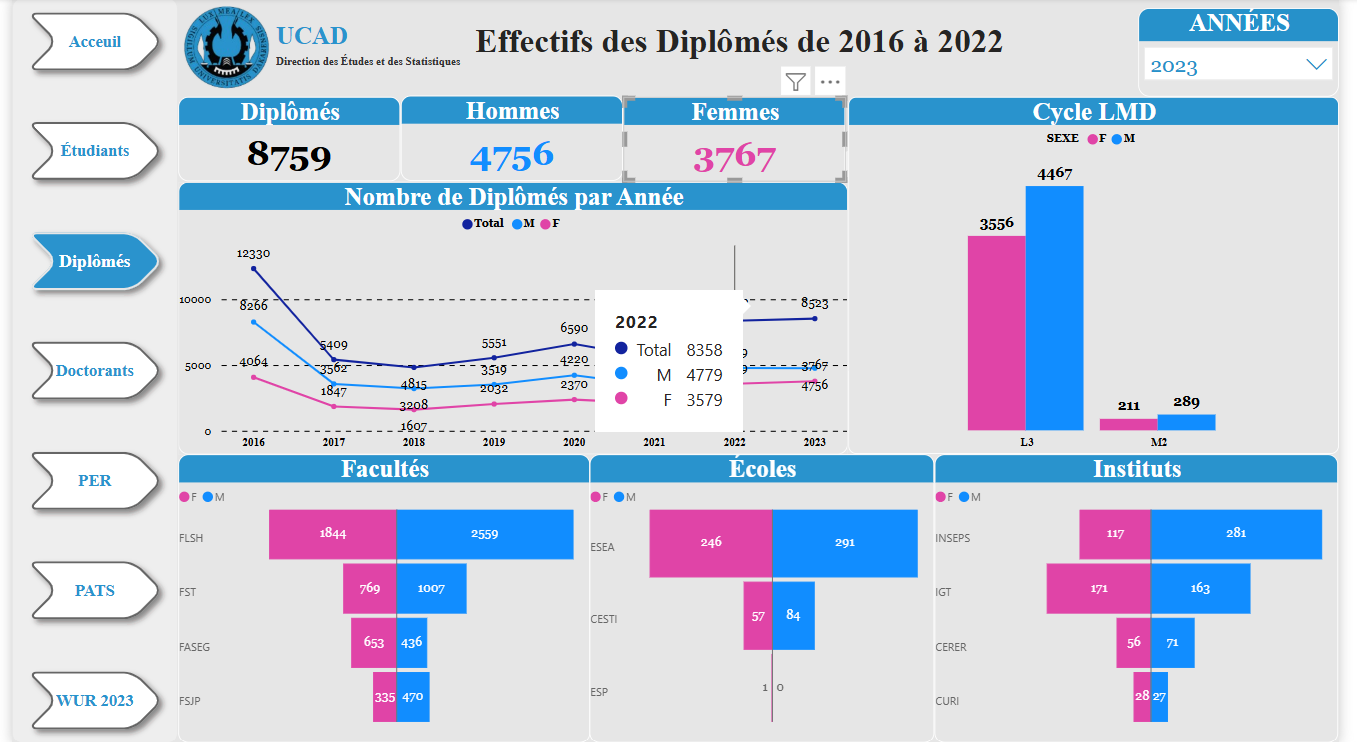
\includegraphics[width=1\textwidth]{image/diplomes.png} 
    \end{center}

    
    \item \textbf{Tableau de bord des doctorants} : Dans cette section, on a créé des graphiques pour explorer les données des doctorants de l'université. On a pu créer des graphiques pour visualiser le nombre de doctorants par année, par école doctorale,  et par genre. Voici quelques insights que nous avons pu obtenir à partir de ces visualisations : 
    
    - Le nombre de doctorants a augmenté au fil des années jusqu'en 2008, ensuite il a diminué jusqu'en 2012, puis il est resté constant jusqu'en 2017 et continue a augmenter jusqu'en 2023. On compte plus de 4500 doctorants avec 2900 hommes et 1562 femmes   pour l'année académique 2023.

    - la majorité des doctorants sont inscrits a l'école doctorale JPEG avec plus de 600 inscription 400 hommes et 200 femmes pour l'année académique 2023-2024. 

    \begin{center}
    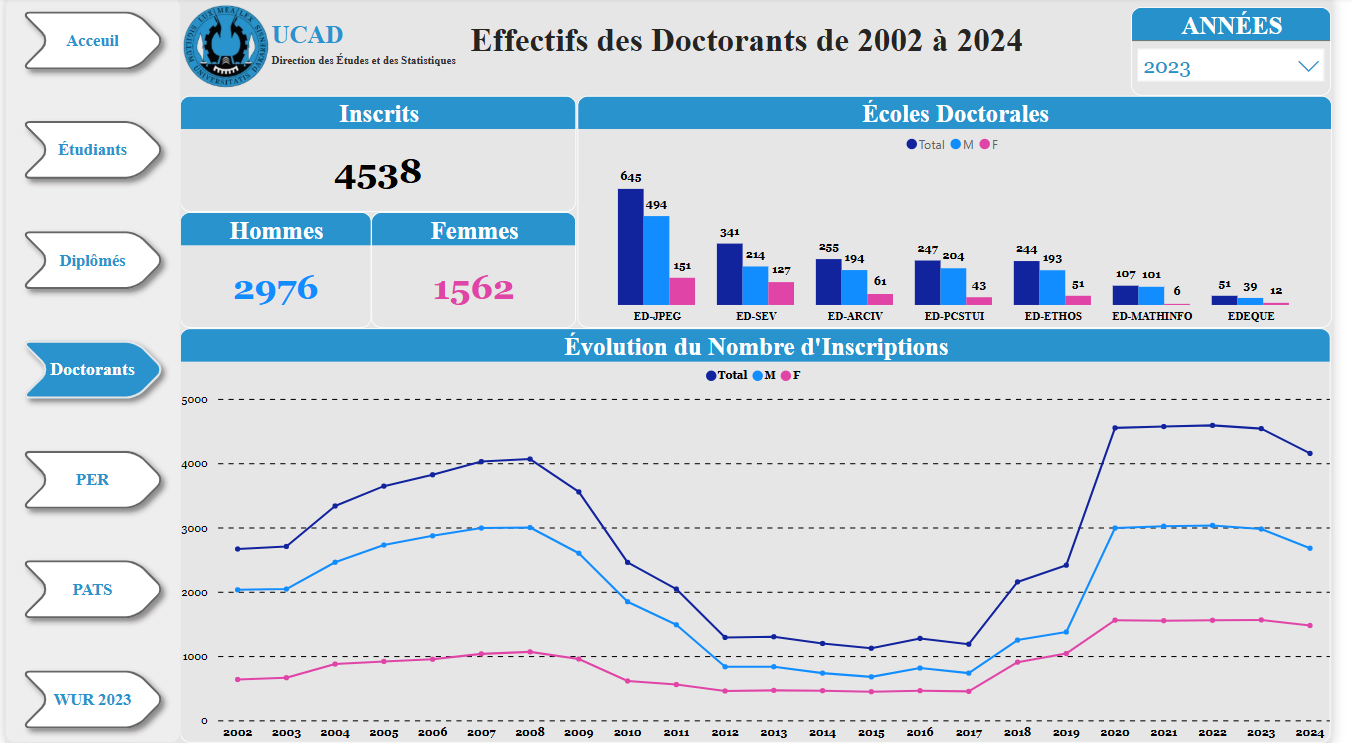
\includegraphics[width=0.9\textwidth]{image/doc.png} 
    \end{center}

  
\end{itemize}     

D'autres visualisations ont été créées pour explorer les données des étudiants, des diplômes et des doctorants. Ces visualisations ont permis de mieux comprendre les tendances et les anomalies dans les données, et de présenter les résultats de manière claire et concise. 


\subsection{Analyse exploratoire des données (EDA)}  
L'analyse exploratoire des données a ete réalise a l'aide de Python et de ses bibliothèques. Elle a permis de comprendre encore plus les les données et de détecter les tendances, les variations saisonnières.
L'objectif de l'EDA est tout d'abord de mieux comprendre la structure des données , de detecter les anomalies et les incohérences deja détectées dans la section précédente , de réaliser des statistiques descriptives et de visualiser les données pour mieux comprendre les tendances et les variations saisonnières et afin de preparer les données pour la modélisation et l'analyse prédictive. 

Pour faire cela j'ai tout d'abord écrit un petit programme en python qui permet de verifier si tous mes fichiers ont les memes colonnes et de les fusionner en un seul fichier
\begin{center}
    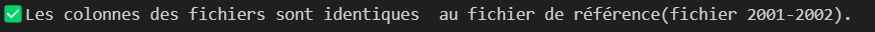
\includegraphics[width=1\textwidth]{image/1.png} 
\end{center} 

Une fois cette étape terminée, j'ai pu concaténer les fichiers en un seul appelé \texttt{df\_total}.\\
Après ces étapes, j'ai pu afficher les 5 premières lignes de mon fichier pour avoir un premier aperçu des données.\\
J'ai aussi utilisé les fonctions \texttt{info()} et \texttt{describe()} pour obtenir des informations sur les colonnes et des statistiques descriptives du fichier.
\begin{center}
    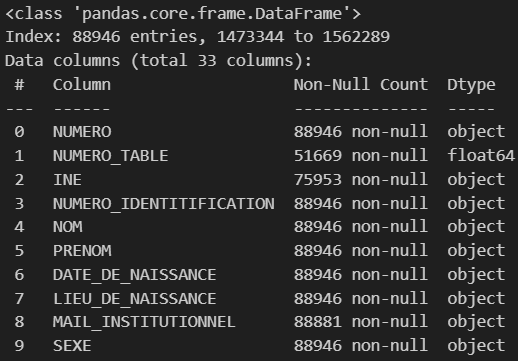
\includegraphics[width=0.5\textwidth]{image/2.png} 
\end{center}  

J'ai ensuite utilisé la fonction \texttt{isnull().sum()} pour vérifier s'il y a des valeurs manquantes dans le fichier. J'ai trouvé qu'il y avait des valeurs manquantes dans certaines colonnes, mais pas dans toutes les colonnes. voici les colonnes manquantes :
\begin{center}
    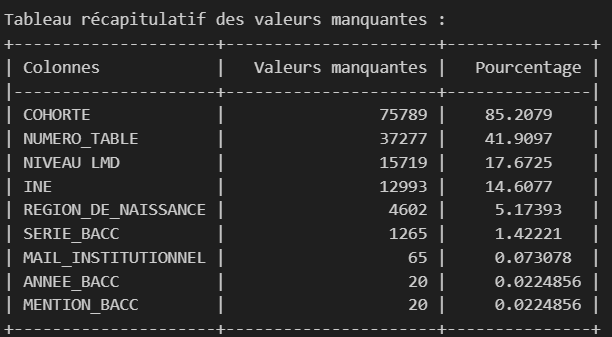
\includegraphics[width=0.5\textwidth]{image/3.png} 
\end{center}  

Apres avoir verifier les valeurs manquantes j'ai créer une autre cellule que j'ai renommé "données démographiques"  pour faire une analyse des données démographiques des étudiants. 
j'ai pu observer l'evolution des effectifs des étudiants au fil des années, la répartition des étudiants par tranche d'age pour l'année 2024  
\begin{center}
    \centering
    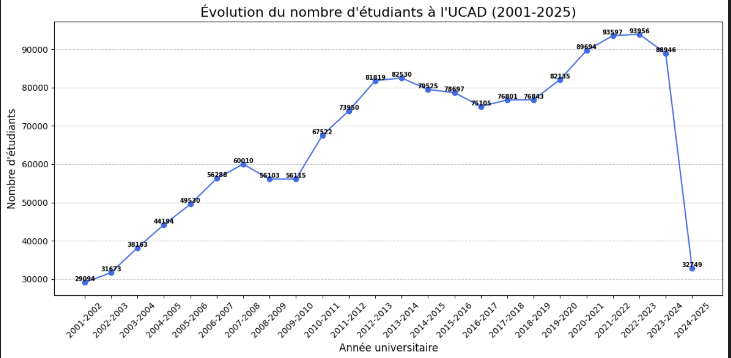
\includegraphics[width=0.45\textwidth]{image/4.png}
    \hspace{0.05\textwidth}
    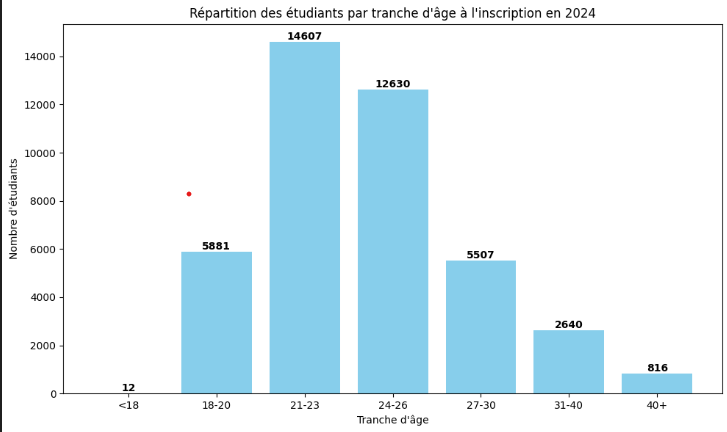
\includegraphics[width=0.45\textwidth]{image/5.png}
\end{center}

\textcolor{red}{\faInfoCircle}\textbf{Conclusion :}  J'ai remarqué que la majorité des étudiants sont âgés de 18 à 25 ans, ce qui est normal car la plupart des étudiants commencent leurs études supérieures à cet âge. Cependant, il y a aussi une proportion importante d'étudiants âgés de 26 à 30 ans, ce qui peut être dû à des étudiants qui ont repris leurs études après une pause ou qui ont changé de filière.
Concernant les inscriptions, j'ai pu observer l'évolution des inscriptions au fil des années. Cependant le nombre d'inscrits est tres basse en 2025 ce qui normale l'année 2024 n'est pas encore terminée. 

\vspace{0.5cm}  

Une fois cette etape termine une autre cellule a été crée pour voir l'historique académique des étudiants. Les différentes series et mentions ont été analysées pour comprendre la répartition des étudiants par série et par mention. J'ai utilisé la fonction \texttt{value\_counts()} pour compter le nombre d'étudiants dans chaque série et chaque mention 
voici les résultats obtenus :
\begin{center}
    \centering
    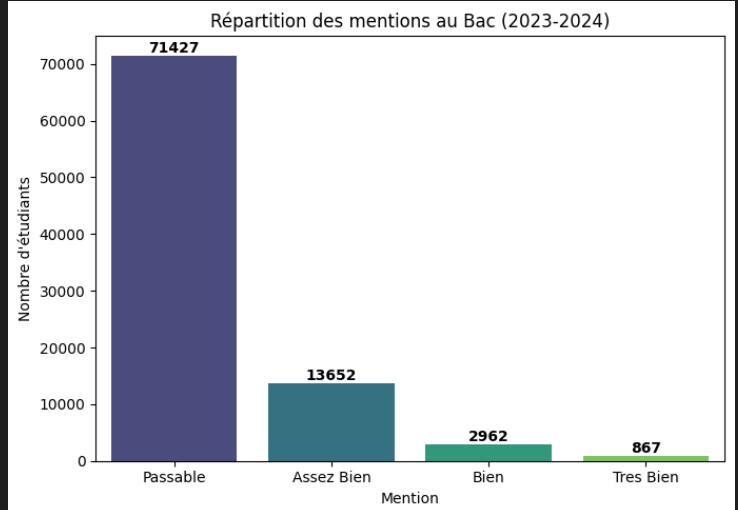
\includegraphics[width=0.45\textwidth]{image/6.png}
    \hspace{0.05\textwidth}
    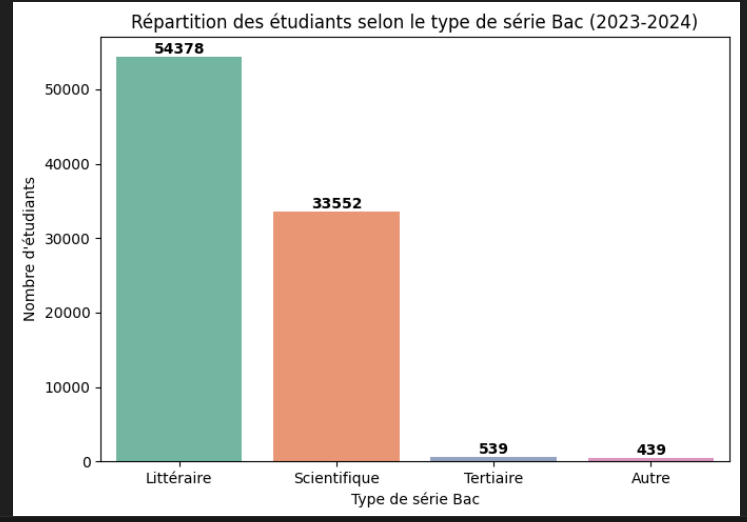
\includegraphics[width=0.45\textwidth]{image/7.png}
\end{center}
\textcolor{red}{\faInfoCircle}\textbf{Conclusion:}  J'ai remarqué que la majorité des étudiants ont obtenu la mention "Passable", suivie de "Assez bien" et "Bien". 
la majorité des étudiants suivent un parcours littéraire(L2 , L1, A , AR etc.. ), suivi des parcours scientifiques(s1 , S2  , D , C ..) et Tertiaire  

j'ai aussi observer le taux de redoublement en première année (l1 ou 1A)pour l'année 2023 est d'environ 19\% ce qui est normal pour une université de cette taille.

j'ai aussi créer une cellule pour voir la proportion des ces  redoublants  par mention et par série du bac voici les résultats obtenus :
\begin{center}
    \centering
    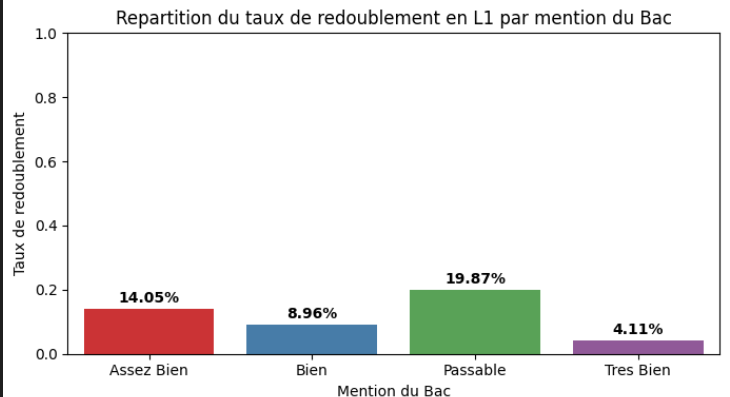
\includegraphics[width=0.45\textwidth]{image/8.png}
    \hspace{0.05\textwidth}
    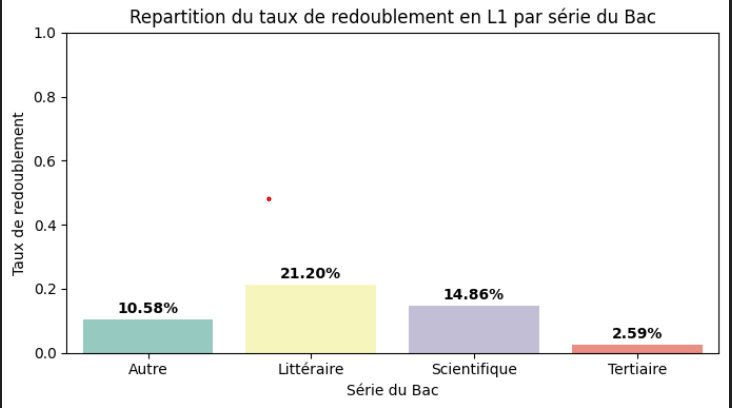
\includegraphics[width=0.45\textwidth]{image/9.png}
\end{center} 

\textcolor{red}{\faInfoCircle}\textbf{Conclusion :}


- effet de la mention du Bac : 
    Les résultats montrent que le taux de redoublement en L1 est d'autant plus élevé que la mention au Bac est faible. Ainsi, les étudiants ayant obtenu la mention "Passable" présentent un taux de redoublement de 19,87\%, contre seulement 4,11\% pour ceux ayant obtenu la mention "Très Bien". De même, les étudiants avec la mention "Assez Bien" connaissent un taux de redoublement relativement élevé 14,05\%, tandis que ceux avec "Bien" affichent un taux plus faible 8,96\%.
Cela montre que la mention du Bac est un indicateur significatif de la réussite en L1, les étudiants ayant de meilleures mentions au Bac étant moins susceptibles de redoubler.

- Effet de la série du Bac : 
L'étude du taux de redoublement selon la série du Bac met en évidence une différence notable entre les profils:

Les étudiants issus des séries littéraires affichent le taux de redoublement le plus élevé 21,20\%, suivis par ceux des séries scientifiques 14,86\% et autres 10,58\%.

Les étudiants issus des séries tertiaires enregistrent le taux le plus bas 2,59\%. Cela suggère que les étudiants des séries littéraires et scientifiques rencontrent plus de difficultés en L1, tandis que ceux des séries tertiaires semblent mieux préparés pour cette étape universitaire. 

Pour verifier si ces résultats sont significatifs, j'ai utilisé le test du Chi-2.
J'ai utilisé la fonction \texttt{chi2\_contingency()} de la bibliothèque \texttt{scipy.stats} pour effectuer le test du Chi-2.
et j'ai constate que la p-value est inférieure à 0.05, ce qui signifie que les résultats sont significatifs.
J'ai donc pu conclure que la mention du Bac et la série du Bac ont un effet significatif sur le taux de redoublement en L1.

\vspace{1cm}  


Une autre analyse appelle suivi de cohorte a ete faite. Le but est de suivre une cohorte d'étudiants sur plusieurs années pour observer leur parcours académique. J'ai créer une fonction qui prend en entrée le jeux de donnée , l'année de bac , la série du bac et l'année universitaire
et qui retourne le nombre d'étudiants qui on redouble pour chaque année universitaire , les diplômes  apres 3 ans 4 ans et 5 ans et le taux d'abandon pour chaque année universitaire. 
Pour une premier version voici les résultats obtenus pour la cohorte de 2019 en série littéraire 
\begin{center}
    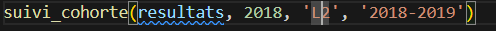
\includegraphics[width=1\textwidth]{image/10.png} 
\end{center} 
\begin{center}
    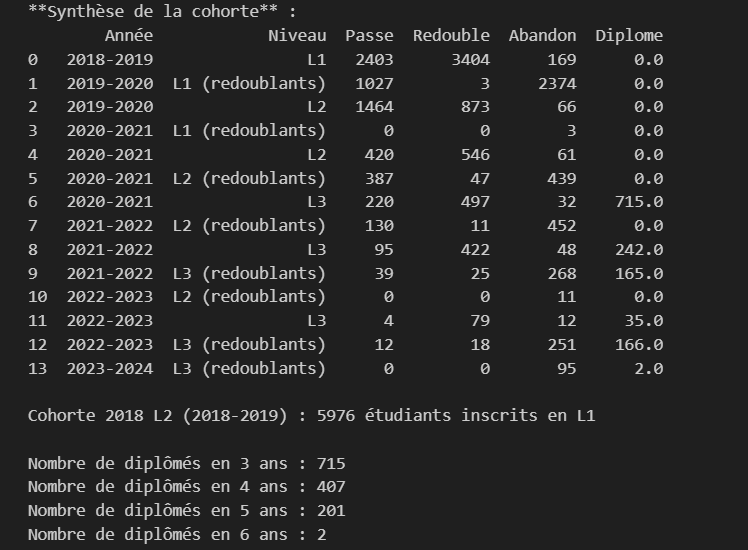
\includegraphics[width=1\textwidth]{image/11.png} 
\end{center} 
Ici, on remarque que sur 5976 inscrits en L1 en 2018-2019, titulaires du baccalauréat série L2 obtenu en 2018, 1325 étudiants ont obtenu leur licence, soit environ 22,2\% de la cohorte initiale.
Parmi eux :
\begin{itemize}
    \item 715 étudiants, soit 53.3\% des diplomes, ont obtenu leur licence en 3 ans,
    \item 407 étudiants, soit 30.7\%, en 4 ans,
    \item 201 étudiants, soit 15.16\%, en 5 ans,
    \item enfin, 2 étudiants, soit environ 0,15\%, en 6 ans.
\end{itemize} 
On remarque  aussi que 77,8\% de cette  cette cohorte n'obtienne pas la license (changement d'ecole  exclusion  voyage , etc...). 

Une deuxième version de cette fonction a été écrite pour faire une analyse plus approfondie des résultats. cette fois si la fonction va prendre en paramètre la faculté et le département de l'étudiant en plus.
\begin{center}
    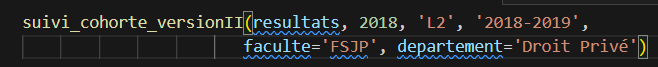
\includegraphics[width=1\textwidth]{image/12.png} 
\end{center} 
\begin{center}
    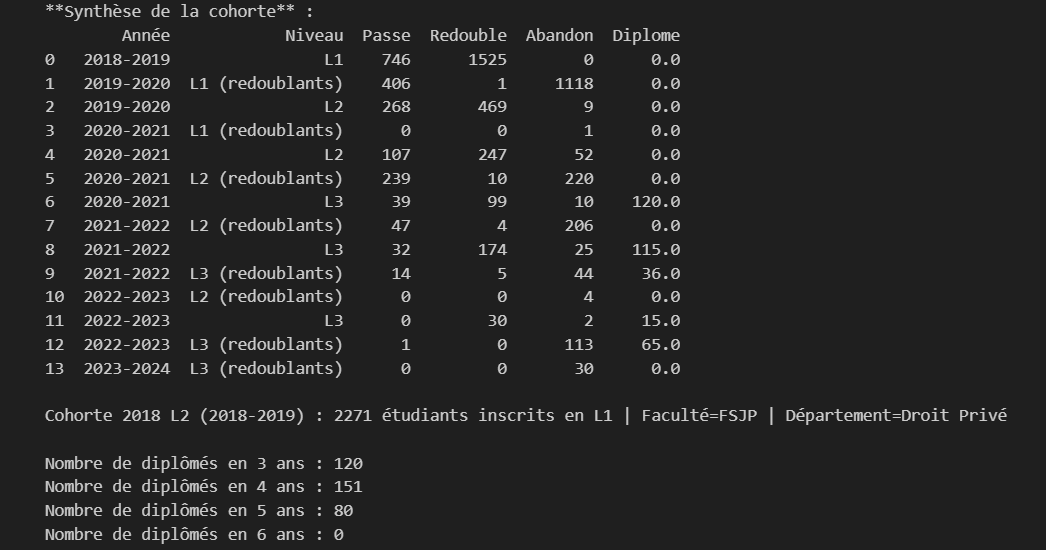
\includegraphics[width=1\textwidth]{image/13.png} 
\end{center} 
\textcolor{red}{\faInfoCircle}\textbf{Conclusion :} 
On remarque que de manière générale le taux de redoublement est relativement élevé. La plupart des étudiants redoublent en L1, suivis de L2 et L3 , et aussi beaucoup d'étudiants abandonnent leurs études en L1.
A noter aussi que une grande partie des étudiants n'obtiennent pas leur licence..Cela peut être dû à plusieurs facteurs, tels que le manque de préparation, les difficultés d'adaptation à l'université , des problèmes personnels ou peut être le système d'orientation qui n'est pas adapté aux étudiants. 

\subsection{Fusion des données}
Je dispose de plusieurs  fichiers 
qui contiennent des informations sur les étudiants c'est a dire leur nom, prénom, date de naissance, numéro d'étudiant, etc.
et leur parcours académiques et un autres fichier contenant les memes données avec les résultats universitaires en plus . J'ai donc decide de fusionner les deux fichiers pour avoir un seul fichier contenant toutes les informations sur les étudiants. 
Pour cela j'ai d'abord sélectionner les colonnes en commun entre les deux fichiers et j'ai utilisé la fonction \texttt{merge()} de la bibliothèque \texttt{pandas} pour fusionner les deux fichiers. 
Pour les fusionner  j'ai utilise la colonne "Numéro" et "Année Université". j'ai utilise le paramètre "inner" pour ne garder que les lignes qui ont des valeurs communes dans les deux fichiers. Une fois la fusion terminée, j'ai vérifié si le nombre de lignes du nouveau fichier était égal à la somme des lignes des deux fichiers d'origine. Apres avoir vérifié que la fusion s'est bien déroulée, j'ai enregistré le nouveau fichier dans un fichier csv appelle \texttt{base\_finale} . 
\begin{center}
    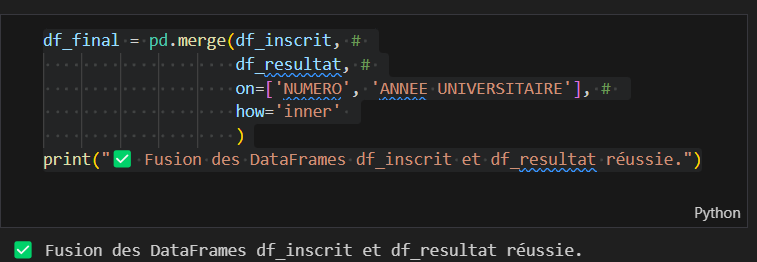
\includegraphics[width=0.7\textwidth]{image/14.png} 
\end{center} 

\subsection{Etude du système DIORES} 
DIORES est un système intelligent d'orientation et de reorientation dans l'enseignement supérieur au Sénégal réalise par des chercheurs et des étudiants  de l'Université Cheikh Anta Diop de Dakar. 
En effet le système actuelle Campusen n'oriente pas efficacement les étudiants dans l'enseignement supérieur. Il ne prend pas en compte des critères comme le profil , les réalités socio-économiques. Il ne propose que les recommandations base sur les données. Ce système n'est pas adapte aux besoins des étudiants car on constate un taux d'échec tres élevé dans l'enseignement supérieur. 
C'est dans ce contexte que l'etude vise a développer un système d'orientation base sur L'IA pour améliorer pour permettre aux étudiants d'être mieux oriente et réoriente dans l'enseignement supérieur. 
Les chercheurs analysent l'écart le classement d'un étudiant de Capusen et sa réussite réelle dans l'enseignement supérieur. 
Les chercheurs analysent l'écart entre le classement d'un étudiant par Campusen et sa réussite réelle dans l'enseignement supérieur, dans le but de proposer un modèle plus fiable. Pour cela, ils ont utilisé  des algorithmes d'apprentissage automatique IA, notamment la régression Lasso et divers modèles de machine learning (régression logistique, forêts aléatoires, réseaux de neurones, etc.)  
Les résultats sont satisfaisant et montrent que le modèle proposé est plus fiable que celui de Campusen. 
Pour avoir un model plus performant et utilisable  les chercheurs envisagent de collecter plus de données sur les étudiants, notamment des données sur leur parcours académique antérieurs , intégrer des variables socio-économiques et psychologiques et enfin Finaliser et déployer une plateforme d'orientation intelligente pour l'enseignement supérieur sénégalais. 
Malheureusement je ne dispose je ne dispose pas des données nécessaire pour reproduire cette etude  

